%this file is drba_gb.tex
\section{Mathematical Background}
\label{sec:background}

In this chapter a mathematical basis is systematically approached to give the reader an understanding of Gröbner Bases and Gröbner fans.\\
In the first section monomials are revisited. The second section explains how monomials can be totally ordered.
After that ideals are defined over polynomial rings and a summary on Gröbner bases and Gröbner fans for ideals is presented. Furthermore, the next sections deal with enumerating Gröbner bases on special ideals. Finally, linear codes are presented and the connection between Gröbner bases and linear codes.  

\subsection{Monomials}
\label{subseb:Monomials}

In this section a brief explanation of polynomials is given.

\begin{env_definition}[Monomial] 
\cite{KHZ}
A monomial is a product of variables over a finite field $\mathbb{K}$, denoted by $ \mathbb{K} \left[X_{1},X_{2},\dots, X_{n}\right]  $ of the form $m= X_{1}^{u_{1}}X_{2}^{u_{2}}\cdots X_{n}^{u_{n}}$, where $u_{i}, 1 < i < n $ and $u \in \mathbb{N}_{0} $
\end{env_definition}
The total \textbf{degree} of a monomial is $deg(m) = \sum_{i=1}^n u_i $. 


\begin{env_definition}[Polynomial]
\cite{KHZ}
A polynomial f is a finite linear combination with coefficients $c_{u} \in \mathbb{K}$ multiplied with monomials.


\begin{align*}
	f &= \sum_{u} c_{u}X^{u} \\
\end{align*}

\end{env_definition}
If $c_{u}\neq0$ then $c_{u}x_{u}$ is a term of $f$.





\subsection{Monomial Order}
\label{subsec:Monomialorder}
It is necessary to rearrange a polynomial with respect to a monomial order. That forms the foundation for dividing polynomials in the finite field
$ \mathbb{K} \left[X_{1},~X_{2},~\dots,~X_{n}\right]~$ and solving the Ideal Membership Problem.\\
The Ideal Membership Problem describes if a polynomial lies in an ideal $I$. Ideals will be defined in section \ref{subsec:Ideals}.

\begin{env_definition}[Term Ordering] 
\cite{saleemi}
A monomial order is a relation $>$ on the set of all monomials in $\mathbb{K}\left[x\right]$.
Let $m_{1}$, $m_{2}$ and $m_{3}$ be monomials
\begin{center}

\begin{itemize}

\item
for any pair of monomials $m_{1}$, $m_{2}$, either $m_{1} > m_{2}$ or $m_{2} > m_{1}$ or $m_{1} = m_{2}$ 
\item
if $m_{1} > m_{2} $ and $m_{2} > m_{3}$ then $m_{1} > m_{3}$
\item
$m_{1} > 1$ for any monomial $m_{1} \neq 1$
\item
if $m_{1} > m_{2}$ then $m \cdot m_{1} > m \cdot m_{2}~$ for any monomial m

\end{itemize}
 
\end{center}

\end{env_definition}


Two commonly used term orders are the following.
Let $u$ and $v$ be elements of $\mathbb{N}^{n}_{0}$. 

\textbf{Lexicographic Order} \cite{saleemi}
$u >_{lex} v $ if in $u-v$ the left most non-zero entry is positive.
This can be written as $X^{u} >_{lex} X^{v}$ if $u >_{lex} v $.\\


\textbf{Graded Lex Order} \cite{saleemi}
$u >_{grlex} v $ if $ deg(u)>deg(v)$ or if $ deg(u)=deg(v)$ and $u >_{lex} v$.

\newpage
\begin{env_example} \normalfont
Let $m_{1} = x^{2}y^{4}z^{3}$ and $m_{2}= x^{1}y^{1}z^{4} \in \mathbb{K}\left[ x,y,z\right]  $.
The monomials can also be written as $m_{1} = X^{(2 \; 4 \; 3)}$ and $m_{2} = X^{(1 \; 1 \; 4)}$.
Thus $m_{1}>_{lex} m_{2}$ because the left most non-zero entry of $ (2 \; 4 \; 3) - (1 \; 1 \; 4)$ is positive.

The total degree of $m_{1}$ is 9 and $deg(m_{2})=6$. Hence, $deg(m_{1})>deg(m_{2})$ so that $m_{1}>_{grlex} m_{2}$ 
\begin{flushright}
$\lozenge$
\end{flushright}
\end{env_example}
  

\textbf{Weight vectors} \\
In order to compare monomials with a generic vector $\left({a}_{1},\dots ,{a}_{n}\right)~\in \mathbb{R}^{n}_{+}~$, the dot product with the exponent vector has to be taken. The highest result is the leading term. If a tie occurs, some other fixed monomial order has to be used. Note that the standard monomial orders can be expressed as weight vector. The lexicographic order needs for instance the first unit vector, if a tie occurs the second unit vector and so on.

\textbf{Leading term}

Given a term order $>$, each non-zero polynomial $f \in \mathbb{K}\left[ x\right] $ has a unique leading term, denoted by $\textsc{LT}(f)$, given by the largest involved term with respect to the term order.\\
If $\textsc{LT}(f) = cX^{u}$, where $c \in \mathbb{K}$, then c is the leading coefficient of $f$ and $X^{u}$ is the leading monomial (\textsc{LM}) or the initial monomial \cite{KHZ}.\\

\begin{env_example}\normalfont

Let $ f = 3x^{2}y^{5}z^{3} + x^{4} -2x^{3}y^{4} + 12x^{2}z^{2}$ \\
With respect to lex order : $f = \underline{x^{4}} -2x^{3}y^{4} + 3x^{2}y^{5}z^{3} + 12x^{2}z^{2} $ \\
with respect to grlex order : $f = \underline{3x^{2}y^{5}z^{3}} -2x^{3}y^{4} + x^{4}+ 12x^{2}z^{2}$  \\
with respect to the weight vector $\left(3,2,1\right)~$: $f = \underline{3x^{2}y^{5}z^{3}} -2x^{3}y^{4} + x^{4}+ 12x^{2}z^{2}$  \\ 
The underlined terms are the leading terms with the respect to the monomial order.
\begin{flushright}
$\lozenge$
\end{flushright} 
\end{env_example}


\newpage
\subsection{Ideals}
\label{subsec:Ideals}

\begin{env_definition}[Ideal]
\cite{KHZ}
An ideal I is a collection of polynomials \\ $f_{1},\dots ,f_{s} \in \mathbb{K}\left[X_{1}, \cdots, X_{n}\right] $ and polynomials which can be built from these by addition and multiplication with arbitrary polynomials.

\end{env_definition}
This is called an ideal generated by $f_{1}, \dots , f_{s}$ \\
\[ \langle f_{1}, \dots , f_{s} \rangle = \left\lbrace  \sum_{i=1}^s h_{i}f_{i} \mid h_{1}, \dots , h_{s} \in \mathbb{K}\left[X_{1}, \dots, X_{n}\right] \right\rbrace \]
\\
An ideal satisfies $\cite{saleemi} $:
\begin{center}

\begin{itemize}
\item
$0 \in I = \langle f_{1}, \cdots , f_{s} \rangle$ 
\item
If $f,g \in \langle f_{1}, \cdots , f_{s} \rangle$,then  $f+g \in \langle f_{1}, \cdots , f_{s} \rangle$ 
\item
If $f \in \langle f_{1}, \cdots , f_{s} \rangle$ and $h \in  \langle f_{1}, \cdots , f_{s} \rangle$, then $f \cdot h \in \langle f_{1}, \cdots , f_{s} \rangle$
\end{itemize}

\end{center}


\begin{env_example}\normalfont
Let $ I= \langle f_{1},f_{2} \rangle = \langle x^{2}+y, x+y+1 \rangle $ and $f=yx^{2}+y^{2}+x^{2}+xy+x$. Since $f= y \cdot f_{1} + x \cdot f_{2}, f\in I$.
\begin{flushright}
$\lozenge$
\end{flushright} 
\end{env_example}


\begin{env_definition}[Leading Ideal]
\label{def:initial}
\cite{tigers} The leading ideal of I with respect to a term order $>$ on $\mathbb{K}\left[X_{1}, \cdots, X_{n}\right]$ is the monomial ideal \\
\[lt_{>}(I) = \langle lt_{>}(f) : f \in I  \rangle . \]

\end{env_definition}
The set $lt_{>}(f)$ means the leading term of $f$ with respect to $>$. In other words, the leading ideal of $I$ is the ideal generated by its leading terms.

\newpage


\subsection{Division Algorithm}
\label{subsec:division}

The Ideal Membership Problem is easy to solve in a polynomial ring with one variable. It is only necessary to apply the polynomial division, which means dividing the polynomial by the ideal and to check if the remainder is zero. 
If the result has zero remainder, the polynomial $p$ lies in the ideal $I$.
But in a ring with several variables like $ \mathbb{K} \left[X_{1},X_{2},\cdots X_{n}\right]$, the usual division algorithm will not work. A generalized algorithm is needed.\\ \\
The goal is to divide $g \in \mathbb{K}\left[X_{1}, \cdots, X_{n}\right] $ by 
$f_{1}, \ldots, f_{s} \in \mathbb{K}\left[X_{1}, \cdots, X_{n}\right]$, so $g~$ can be expressed in the form \begin{center}
$g = a_{1}f_{1}+ \ldots + a_{s}f_{s} +r$
\end{center} 
where the $a_{1}f_{1}+ \ldots + a_{s}f_{s} $ and $r \in \mathbb{K}\left[X_{1}, \cdots, X_{n}\right]$ $\cite{coxOshea}$.
The remainder $r~$is zero or $r~$is a linear combination with the coefficients in $\mathbb{K}$, none of them are divisible by any of
$\textsc{LT}\left(f_{1} \right), \ldots, \textsc{LT}\left(f_{s} \right)  $.
Furthermore, if $a_{i}f_{i} \neq 0 $, then
$deg(g) \geq deg(a_{i}f_{i})$.

\newpage


\begin{algorithm}
\caption{Division Algorithm \cite{KHZ}}
\label{alg:division}
\begin{algorithmic}[1]

\Require Basis $\langle f_{1}, \cdots, f_{m}\rangle$ of nonzero polynomials  
\Ensure $r=0$ or none of the terms in $r$ are divisible by $ LT_{\leq}\left( f_{1}\right) , \cdots , LT_{\leq} \left( f_{m}\right) $

\State $ h_{1} \gets 0 ,~\cdots ,~h_{m} \gets 0;~r \gets 0;~s \gets f  $

\While{$s \neq 0$}
\State $ i \gets 1 $
\State  division\textunderscore occured $ \gets $  false 
\While{$i\leq m$  and division\_occured = false}
\If{$LT\left( f\left[ i\right] \right)$ divides $LT\left( s\right)  $}

\State $ s \gets s - ( LT \left( s\right)/ LT \left( f \left[ i\right] \right))  \cdot f_{i} $
\State $h_{i} \gets h_{i} + LT\left( s\right) / LT\left( f_{i}\right) $
\State division\textunderscore occured = true
\Else
\State $i \gets i+1$
\EndIf
\EndWhile

\If{division\textunderscore occured = false}
\State $ r \gets r + \textsc{LT}\left( s\right) $
\State $ S \gets s - \textsc{LT}\left( s\right) $
\EndIf

\EndWhile


%\EndProcedure
\end{algorithmic}
\end{algorithm}


\begin{env_example}\normalfont
Consider the ideal $I = \langle f_{1},f_{2} \rangle = \langle xy^{2}+z,y^{2}-1 \rangle~$and the polynomial $f = x^{3}y^{2}+x^{2}z~$.
First, with respect to the lex-order, applying the division gives the expression : $f = x^{2}(xy^{2}+z) + 0(y^{2}-1) + 0$ \\
But the division with $f$ and $I = \langle f_{2},f_{1} \rangle$ gives the expression \\ $f = x^{3}(y^{2}-1) + x^{2}(xy^{2}+z) -x^{3}y^{2}+x^{3}~$.
\begin{flushright}
$\lozenge$
\end{flushright}
\end{env_example}



This example shows that is still possible to obtain a non-zero remainder even if $f \in \langle f_{1},f_{2} \rangle $. That means r = 0 is a  necessary condition for the ideal membership but not a sufficient condition.
\subsection{Gröbner basis}
\label{subsec:Groebner}

The solution of the Ideal Membership Problem needs a certain generating set for an ideal $I$. It would be helpful if the remainder $r$ on division is uniquely determined and the condition $ r = 0~$ is equivalent to the membership in the ideal.



\begin{env_definition}[Gröbner basis]
\cite{KHZ}
Let $\leq$ be a monomial order on \\ $\mathbb{K}\left[X_{1}, \cdots, X_{n}\right]$ and let I be an ideal on $ \mathbb{K}\left[X_{1}, \cdots, X_{n}\right]  $. A Gröbner basis G for I (with respect to $\leq$) is a finite set of polynomials $ G = \left\lbrace f_{1}, \ldots , f_{m} \right\rbrace $ in I with the property that for every nonzero $ f \in I , \textsc{LT}_{\geq}(f) $ is divisible by $\textsc{LT}\left( f_{i}\right) $ for some $ 1 \leq i \leq m $.

\end{env_definition}

A Gröbner basis has the beneficial property that the remainder $r$ of $f$ by the elements of a Gröbner basis are uniquely determined and independent of the order of the elements in $G$.
Also every ideal in $\mathbb{K}\left[X_{1}, \cdots, X_{n}\right]$ has a Gröbner basis with respect to any monomial order\cite{KHZ}.\\ 


In order to obtain a Gröbner basis of an arbitrary basis $\{f_{1}, \ldots , f_{n}\}$ with an arbitrary monomial order $>$ of an ideal $I$, an algorithm is needed. This algorithm is called Buchberger-Algorithm. The idea is to build every possible S-Polynomial of $\left( f_{i},f_{j}\right) $ for every $ 1 \leq i \neq j \leq n $ and every nonzero result is added to the basis until every S-Pair of $\left( f_{i},f_{j}\right) $ vanishes.

Let the polynomials $f,g \in \mathbb{K}\left[X_{1}, \cdots, X_{n}\right] $ and $\textsc{LT}_{\leq}\left(f \right) = cX^{\upalpha} $, \\  $\textsc{LT}_{\leq}\left(g \right) = dX^{\upbeta} $ and $\textsc{LCM}\left( X^{\upalpha},X^{\upbeta}\right) $ be the least common multiple between $X^{\upalpha}$ and $X^{\upbeta}$. 

\begin{env_definition}[S-Polynomial]
\cite{KHZ} The S-polynomial of f and g is the polynomial

\[ S\left( f,g\right) = \frac{\textsc{LCM}\left( X^{\upalpha}, X^{\upbeta}\right) }{\textsc{LT}_{\leq}\left( f\right) } \cdot f - \frac{ \textsc{LCM}\left( X^{\upalpha}, X^{\upbeta}\right) }{\textsc{LT}_{\leq}\left( g\right) } 
\cdot g. \]


\end{env_definition}

\newpage

\begin{env_example}\normalfont
Consider the polynomials the polynomial ring $\mathbb{K}\left[ x,y,z\right] $ with
the basis $\left\lbrace f,g\right\rbrace = \left\lbrace xy^{2}-xz+y,xy-z^{2} \right\rbrace $ with respect to the lexicographic order.\\
Forming the S-Polynomial leads to:

\begin{align*}
 S \left(f,~g\right) &= \dfrac{\textrm{LCM}\left( xy^{2}, xy \right) } {xy^{2} } \cdot \left(  xy^{2}-xz+y\right) - \dfrac{\textrm{LCM}\left( xy^{2},~xy \right) } {xy } \cdot \left( xy-z \right) \\ 
 &= \dfrac{xy^{2}}{xy^{2}} \cdot \left( xy^{2}-xz+y\right) - \dfrac{xy^{2}}{xy} \cdot \left( xy-z\right) \\
 &= -xz-yz+y 
\end{align*}


\begin{flushright}
$\lozenge$
\end{flushright} 
\end{env_example}

The S-Polynomial is not zero and is not divisible by the leading terms of $f$ or $g$. That means the basis given in the example is not a Gröbner basis. This can be deduced by the following assertion.

\begin{env_definition}[Buchberger Criterion]
\cite{KHZ} A finite set $G = \left\lbrace f_{1}, \cdots , f_{m} \right\rbrace$ of polynomials in $ \mathbb{K}\left[X_{1}, \cdots, X_{n}\right] $ is a Gröbner basis of an ideal 
$I = \langle f_{1}, \cdots , f_{m} \rangle $ if and only $S\left( f_{i},f_{j}\right) = 0$, $ \forall$  $1 \leq i,j \leq n, i\neq j $

\end{env_definition}

\begin{algorithm}
\caption{Buchbergers Algorithm \cite{KHZ}}
\label{alg:buchberger}
\begin{algorithmic}[1]
%\Procedure{Euclid}{$a,b$}\Comment{The g.c.d. of a and b}
\Require Basis $F = \left( f_{1}, \cdots, f_{m} \right)  $
\Ensure Gröbner basis $G$ for $I = \langle f_{1}, \cdots, f_{m} \rangle $ with $ F \subseteq G $
\State $G \gets F$
\Repeat
\State $G'\gets G $
\For{each pair $f_{i}$ and $f_{j}$ in $G$ , $i\neq j$ }
\State $S \gets S\left( f_{i},f_{j} \right)^{G'}  $ \Comment{S-Polynomial with the basis of $G'$ }
\If{$G\neq 0$ }
\State $G \gets G \cup \left\lbrace S\right\rbrace $
\EndIf
\EndFor
\Until{$G = G'$}

%\EndProcedure
\end{algorithmic}
\end{algorithm}

This algorithm is correct and terminates.\cite{KHZ}

\newpage

However, a Gröbner basis is not unique. A arbitrary polynomial can be added to a Gröbner basis and will remain a Gröbner basis.
Fortunately, each nonzero ideal in $\mathbb{K}\left[X_{1}, \cdots, X_{n}\right]$ has a unique \textit{reduced} Gröbner basis with respect to a fixed monomial order.

%% monic polynomial := Leading coefficient = 1
\begin{env_definition}[Reduced Gröbner basis]
\cite{KHZ}
A Gröbner basis \\ $G= \left\lbrace  f_{1}, \cdots , f_{m} \right\rbrace  $ in 
$ \mathbb{K}\left[X_{1}, \cdots, X_{n}\right] $ is reduced if the polynomials $f_{1},\cdots , f_{m} $ are monic and no term $f_{i}$ is divisible by $ \textsc{LT}_{\leq }\left( f_{j}\right)$ for any pair $i\neq j$, where $\leq$ is monomial order.
\end{env_definition}


\subsection{Gröbner fans}
\label{subsec:Groebnerfan}
 Gröbner bases for a fixed ideal $I$ with different monomial orders can look very different and have different properties. The difference can be in the number of elements in the Gröbner basis, the size or the degree of the elements. So it will be helpful if all 
possible Gröbner basis of a fixed ideal can be collected together.\\
Even though there are infinite monomial orders for an ideal, the amount of reduces Gröber bases are finite \cite{coxOshea}. 
 
\begin{env_definition}[Gröbner fan]
\cite{coxOshea} A Gröbner fan of an ideal $I$ consists of finitely many closed convex polyhedral cones with vertices at the origin, such that

\begin{itemize}
\item
A face of a cone $\sigma$ is $\sigma \cap \lbrace l=0\rbrace$, where $l=0$ is a nontrivial linear equation such that $l \geq 0$ on $\sigma$.
Any face of a cone in the fan is also in the fan.
\item
The intersection of two cones in the fan is a face of each.
\end{itemize}

\end{env_definition}

In order to construct a Gröbner fan to a given ideal, consider the marked Gröbner basis $G = \lbrace g_{1},\cdots,g_{t}\rbrace $ of the ideal $I$.
A marked Gröbner basis is a Gröbner basis where each $g \in G$ has an identified leading term, such that G is a reduced Gröbner basis with respect to some monomial order $>$ selecting those terms.
Informally, where all leading terms in G are marked.\\
\newline
The elements of G, $g_{i}~$, can be written as
\begin{align*}
 g_{i} &  = x^{\upalpha\left( i\right) } +  \sum_{\upbeta} c_{i,\upbeta} \cdot x^{\upbeta}, 
\end{align*}
where $ x^{\upalpha\left( i\right) }$ is the leading term and $ x^{\upalpha\left( i\right) } > x^{\upbeta} $, with respect to a monomial order, whenever $c_{i,\upbeta} \neq 0 $.

If a weight vector $\textbf{w}$ satisfies the inequality
$\upalpha\left( i\right) \ast \textbf{w} \geq \upbeta~\ast\textbf{w}$, the vector selects the correct leading term in $g_{i}$ as the term with the highest weight.\\

So, the cone of a Gröbner basis can be written as \cite{coxOshea}\\
\begin{center}
$C_{G} = \left\lbrace \textbf{w} \in \left(\mathbb{R}^{n}\right)^{+} : \upalpha\left( i\right) \cdot \textbf{w} \geq \beta \cdot \textbf{w}~~~ \textrm{whenever}~ c_{i,\upbeta} \neq 0 \right\rbrace   $
\end{center}


\begin{env_example}\normalfont
\label{ex:groebnerfan}
Consider the ideal with $ I = \langle x^{2}-z,y-x \rangle \in \mathbb{Q}\left[ x,y,z\right] .$
Note that the ring has 3 variables so that Gröbner fan can be plotted in the positive orthant $ \mathbb{R}^{3}_{+}$. \\
The marked Gröbner basis with respect to the \textit{lex} order with $x>y>z$ is
\begin{center}
$G^{\left( 1\right) } = \left\lbrace \underline{y^{2}}-z,\underline{x} -y\right\rbrace $
\end{center}
The leading terms are underlined. Let $\textbf{w} = \left( a,b,c\right) \in \mathbb{R}^{3}_{+} $. Then \textbf{w} is in the cone $C_{G^{1}}$ if and only if the inequalities defined above are satisfied.

\begin{itemize}

\item
$\left( 2,0,0\right) \cdot \left( a,b,c\right) \geq \left( 0,0,1\right) \cdot \left( a,b,c\right) $ or $2a\geq c$ 
\item
$\left( 0,1,0\right) \cdot \left( a,b,c\right) \geq \left( 0,0,1\right) \cdot \left( a,b,c\right) $ or $b\geq a$ 

\end{itemize} 

This is the first cone of the Gröbner fan and can be drawn in the positive orthant. It is sliced of the plane of $a+b+c=d~,d\in \mathbb{R}_+$ for a better clarity.


\begin{figure}
    \centering
    \begin{subfigure}[b]{0.48\linewidth}        %% or \columnwidth
        \centering
        

%nicht kompletter Groebner fan

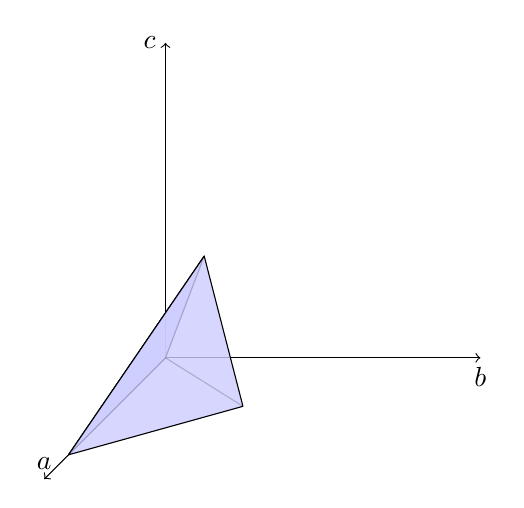
\begin{tikzpicture}[join=round,scale=0.8]
    \tikzstyle{conefill} = [fill=blue!20,fill opacity=0.8]
    \tikzstyle{ann} = [fill=white,font=\footnotesize,inner sep=1pt]
    \tikzstyle{ghostfill} = [fill=white]
    \tikzstyle{ghostdraw} = [draw=black!50]
    
    \draw[arrows=->,line width=.4pt](0,0,0)--(0,0,5); %Z_achse
    \draw[arrows=->,line width=.4pt](0,0,0)--(0,5,0); %Y-ACHSE
    \draw[arrows=->,line width=.4pt](0,0,0)--(5,0,0); %X-ACHSE
    %\draw[arrows=<-,line width=.4pt](.42,-.767)--(4,-2);
    
    \path (5,0,0) node[below] {$b$} (0,0,5) node[above] {$a$} (0,5,0) node[left] {$c$};
    
% letzte Koordinate ist A!!!
% zweite Koordinate ist C!!!
% dritte Koordinate ist B!!!
  
\filldraw[conefill](0,0,0)--(0,0,4)--(1,2,1)--cycle;
\filldraw[conefill](1,2,1)--(0,0,4)--(2,0,2)--cycle;
%\filldraw[conefill](1,2,1)--(0,0,0)--(2,0,2)--cycle;

\draw [opacity=0.2] (0,0,0) -- (2,0,2) ;
 
   
\end{tikzpicture}
        \caption{Gröbner cone for the first basis}
        \label{fig:singlegroebner}
    \end{subfigure}
    \begin{subfigure}[b]{0.48\linewidth}        %% or \columnwidth
        \centering
        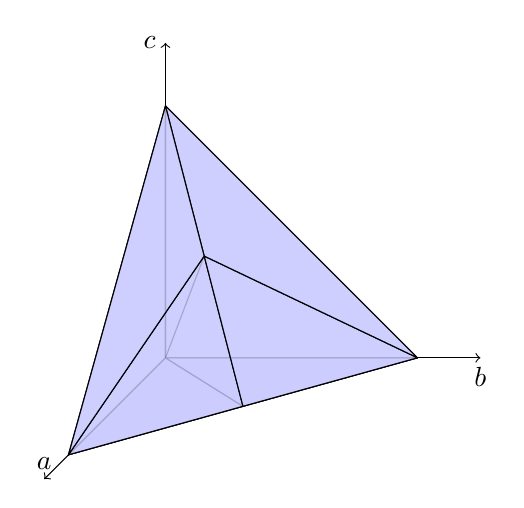
\begin{tikzpicture}[join=round,scale=0.8]
    \tikzstyle{conefill} = [fill=blue!20,fill opacity=0.8]
    \tikzstyle{ann} = [fill=white,font=\footnotesize,inner sep=1pt]
    \tikzstyle{ghostfill} = [fill=white]
    \tikzstyle{ghostdraw} = [draw=black!50]
    
    \draw[arrows=->,line width=.4pt](0,0,0)--(0,0,5); %Z_achse
    \draw[arrows=->,line width=.4pt](0,0,0)--(0,5,0); %Y-ACHSE
    \draw[arrows=->,line width=.4pt](0,0,0)--(5,0,0); %X-ACHSE
    %\draw[arrows=<-,line width=.4pt](.42,-.767)--(4,-2);
    
    \path (5,0,0) node[below] {$b$} (0,0,5) node[above] {$a$} (0,5,0) node[left] {$c$};
   
% erste Koordinate ist B!!! 
% zweite Koordinate ist C!!!   
% dritte Koordinate ist A!!!


% äußere Flächen!

\filldraw[conefill](0,0,0)--(0,4,0)--(0,0,4)--cycle;
\filldraw[conefill](0,0,0)--(4,0,0)--(0,0,4)--cycle;
\filldraw[conefill](0,0,0)--(4,0,0)--(0,4,0)--cycle;

% untenfläche
\filldraw[conefill](0,0,0)--(0,0,4)--(2,0,2)--cycle;
\filldraw[conefill](0,0,0)--(4,0,0)--(2,0,2)--cycle;

%
\filldraw[conefill](0,0,4)--(2,0,2)--(1,2,1)--cycle;
\filldraw[conefill](4,0,0)--(2,0,2)--(1,2,1)--cycle;

\filldraw[conefill](4,0,0)--(1,2,1)--(0,4,0)--cycle;
\filldraw[conefill](0,0,4)--(1,2,1)--(0,4,0)--cycle;

% zur Übersichtlichkeit die gerade im "inneren" des Cones
\draw [opacity=0.2] (0,0,0) -- (1,2,1) ;
\end{tikzpicture}
        \caption{Complete Gröbner fan}
        \label{fig:completegroebner}
    \end{subfigure}
    \caption{Gröbner fans for the given example}
    \label{fig:groebnerfans}
\end{figure}




Figure \ref{fig:singlegroebner} shows that the Gröbner fan is not complete, since the cone does not cover the whole positive orthant. In this example, the other reduced Gröbner basis can be obtained by applying the Buchberger-Algorithm with common term orders to the ideal $I$.
If the computed cones still are not the the whole positive orthant, then a further computation with weight vectors are necessary.
\begin{flushright}
$\lozenge$
\end{flushright} 
\end{env_example}

The example illustrates clearly that an arbitrary non-negative weight vector can be selected and if the vector lies in a certain cone, the corresponding Gröbner base will match with respect to this weight vector.  


This strategy is reasonable for small examples like above.
In genearal, the whole Gröbner fan can be computed with the Gröbner walk \cite{coxOshea}.\\
An inexpensive way to obtain all reduced Gröbner bases of a special ideal, the Code ideal, will be explained in section \ref{subsec:enumerate}.

\newpage
\subsection{Toric Ideals}
\label{subsec:toric}
This work is focused on Code Ideals, so it is useful to define toric ideals first. Given a matrix $A =\left[a_{1},\dots, a_{n}  \right] \in \mathbb{Z}^{d \times n } $ and $u \in \mathbb{Z}^{n}$, which can be decomposed in $u^{+} $ and $u^{-}$, where $u^{+} $ and $u^{-}$ have non-negative coefficients and disjoint support.

\begin{env_definition}[Toric Ideal]
\cite{dueckjournal} A toric ideal $I_{A}$ is defined as
\begin{center}
$ \textbf{I}_{A} = \langle \textbf{x}^{u^{+}} - \textbf{x}^{u^{-}} \mid u \in ker \left(  A \right) \rangle  $
\end{center}


\end{env_definition}

The toric ideal can also be expressed as
\begin{center}
$ \textbf{I}_{A} =  \langle \textbf{x}^{u} - \textbf{x}^{v} \mid Au = Av,~ u,v \in \mathbb{N}^{n}_{0} \rangle .$
\end{center}

\newpage



